\documentclass[fleqn]{article}
\usepackage[spanish,es-noshorthands]{babel}
\usepackage[utf8]{inputenc} 
\usepackage[papersize={6.5in,8.5in},left=1cm, right=1cm, top=1.5cm, bottom=1.7cm]{geometry}
\usepackage{mathexam}
\usepackage{amsmath}
\usepackage{graphicx}

\ExamClass{
\includegraphics[height=16pt]{Images/logo-sed.png} Matemáticas $9^{\circ}$}
\ExamName{``Áreas y volúmenes 2''}
\ExamHead{
\includegraphics[height=16pt]{Images/logo-colegio.png} IEDAB}
\newcommand{\LineaNombre}{%
\par
\vspace{\baselineskip}
Nombre:\hrulefill \; Curso: \underline{\hspace*{48pt}} \; Fecha: \underline{\hspace*{2.5cm}} \relax
\par}
\let\ds\displaystyle

\begin{document}
\ExamInstrBox{
Respuesta sin justificar mediante procedimiento no será tenida en cuenta en la calificación. Escriba sus respuestas en el espacio indicado. Tiene 45 minutos para contestar esta prueba.}
\LineaNombre
\begin{enumerate}
 \item ¿Cuántas caras, vértices y aristas tienen los siguientes prismas? ¿Se cumple el teorema de Euler $V+C-A=2$?
 
 \begin{minipage}{.35\textwidth}
  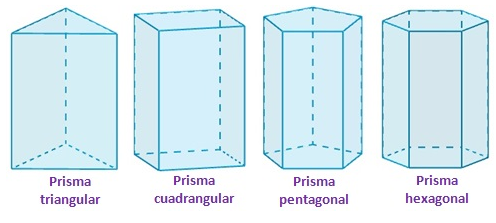
\includegraphics[scale=0.275]{Images/Pantallazo-2017-07-10_19-49-43.png} 
 \end{minipage}\hfill
 \begin{minipage}{.6\textwidth}
 \begin{tabular}{|c|c|c|c|c|}
 \hline 
 Prisma & Caras & Vértices & Aristas & T. de Euler\\ 
 \hline 
 Pentagonal &  &  & & \\ 
 \hline 
 Triangular &  &  &  &\\ 
 \hline 
 Hexagonal &  &  & & \\ 
 \hline 
 Cuadrangular &  &  & &  \\ 
 \hline 
 \end{tabular} 
 \end{minipage}
 \item Un mueble archivador tiene forma de cubo cuya arista mide
60 cm. Calcula los metros cuadrados de madera que se necesitan para construirlo.\noanswer
\item Calcula el área y el volumen de un prisma cuadrado sabiendo que la arista de la base mide 8 cm y la altura 9 cm.\noanswer
\newpage
\item Calcula el área y el volumen de un ortoedro sabiendo que sus dimensiones son 3, 4 y 6 cm.\noanswer
\item Calcula el área y el volumen de un cilindro que tiene radio de la base 6 cm y altura 10 cm\noanswer
 \end{enumerate}
\end{document}
